\section{Muhammad Abdul Gani Wijaya (117407)}
\subsection{Instalasi Map Server dan Map Proxy}
\begin{enumerate}
	\item Buka web mapserver.org
		\begin{figure}[H]
			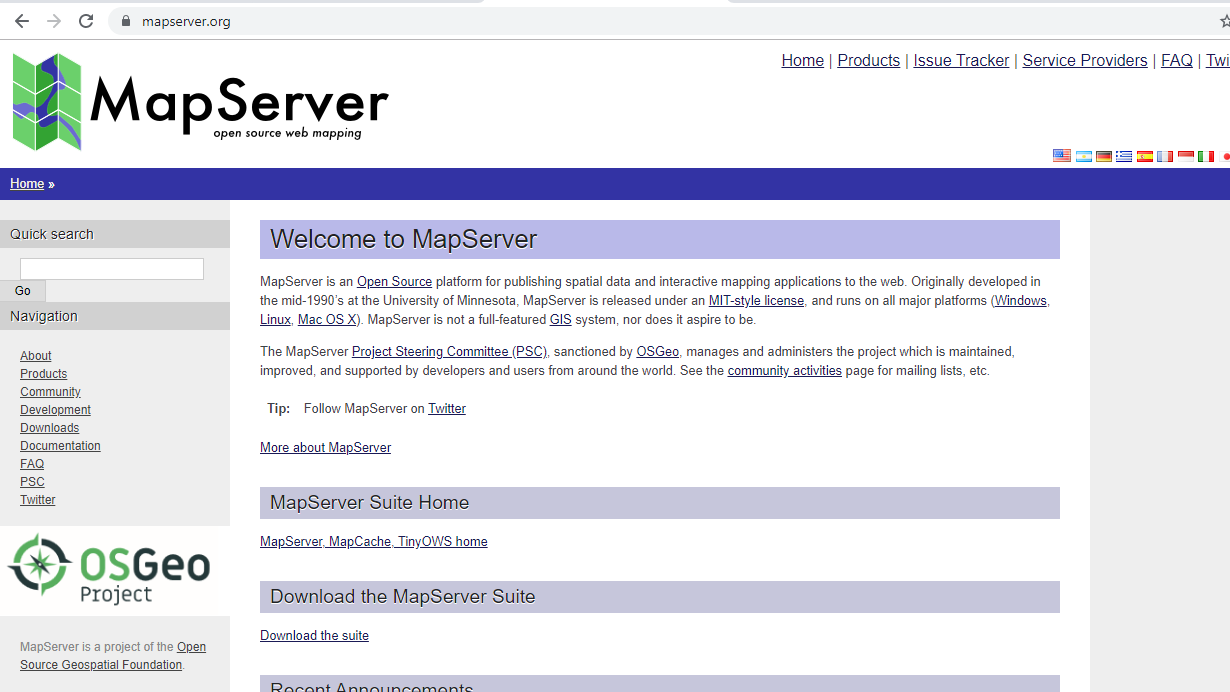
\includegraphics[width=6cm]{figures/Tugas4/1174071/1.png}
			\centering
			\caption{Pilih menu download}
		\end{figure}
	\item Download aplikasi map server untuk window MS4W
		\begin{figure}[H]
			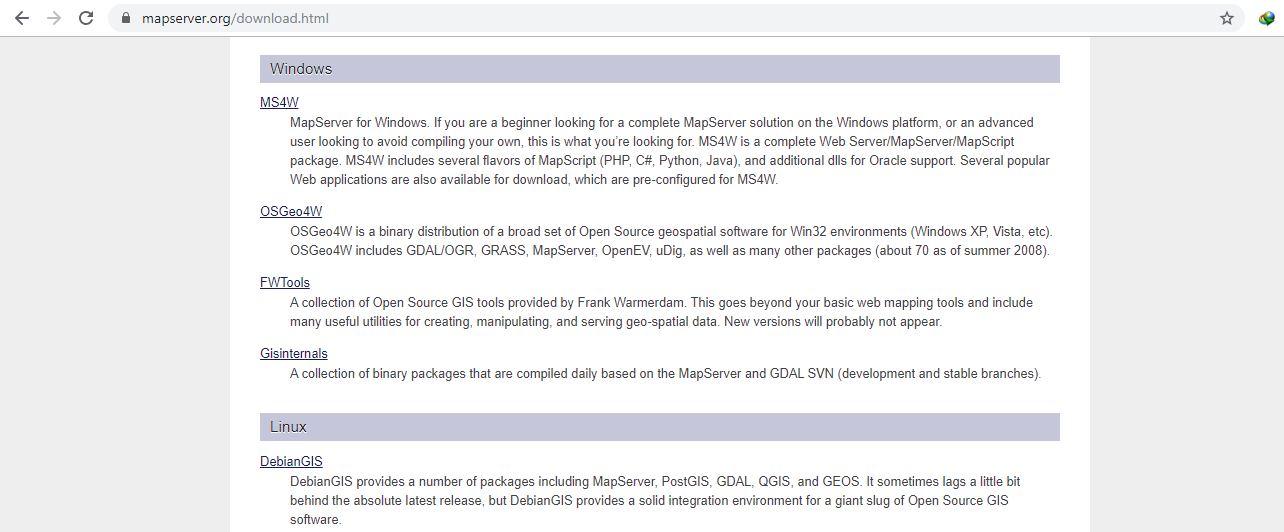
\includegraphics[width=6cm]{figures/Tugas4/1174071/2.png}
			\centering
			\caption{Download aplikasi MS4W}
		\end{figure}
	\item Install aplikasi MS4W
		\begin{figure}[H]
			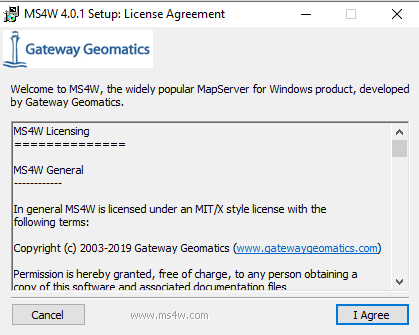
\includegraphics[width=6cm]{figures/Tugas4/1174071/3.png}
			\centering
			\caption{Klik "I Agree" lalu install seperti biasa}
		\end{figure}
	\item Lalu install map proxy dengan perintah 'pip install mapproxy' pada console
		\begin{figure}[H]
			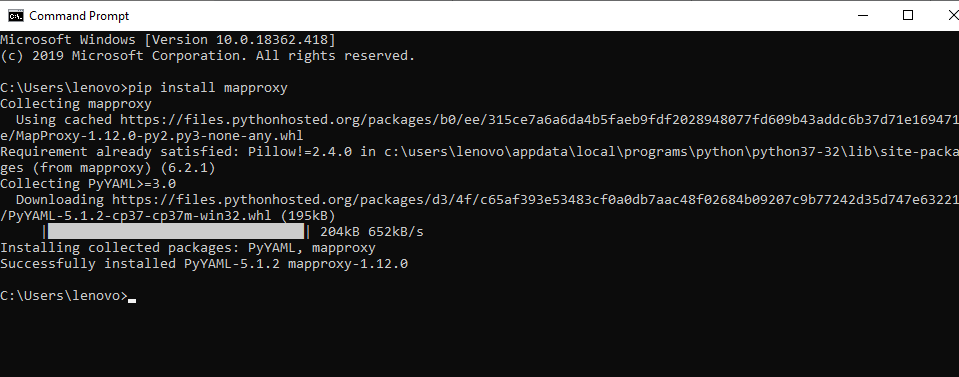
\includegraphics[width=6cm]{figures/Tugas4/1174071/4.png}
			\centering
			\caption{Install mapproxy}
		\end{figure}
	\item Install pyproj dengan perintah 'pip install pyproj' pada console
		\begin{figure}[H]
			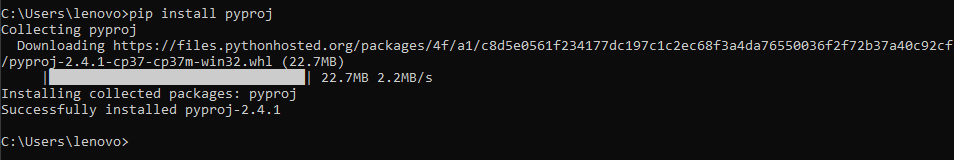
\includegraphics[width=6cm]{figures/Tugas4/1174071/4a.png}
			\centering
			\caption{Install pyproj}
		\end{figure}
		\item Lalu buka service.msc
		\begin{figure}[H]
			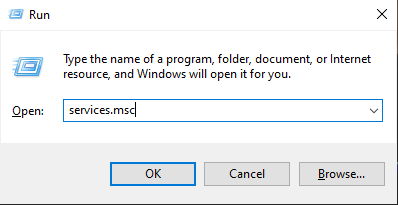
\includegraphics[width=6cm]{figures/Tugas4/1174071/4b.png}
			\centering
			\caption{Membuka service}
		\end{figure}		
		\item Pastikan Apache MS4W Web Server berjalan Automatic
		\begin{figure}[H]
			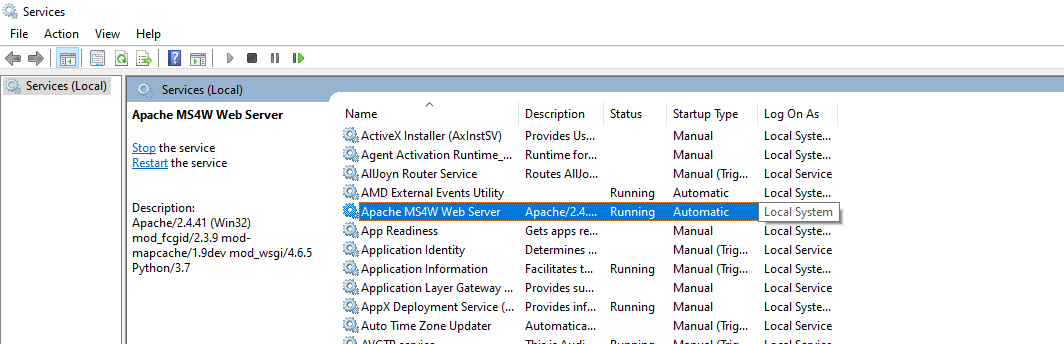
\includegraphics[width=6cm]{figures/Tugas4/1174071/4c.png}
			\centering
			\caption{MS4W Web Server Automatic}
		\end{figure}
\end{enumerate}


\subsection{Pengujian Map Server dan Map Proxy}
\begin{enumerate}
	\item Buka situ http://github.com/awangga/gede lalu download repository
		\begin{figure}[H]
			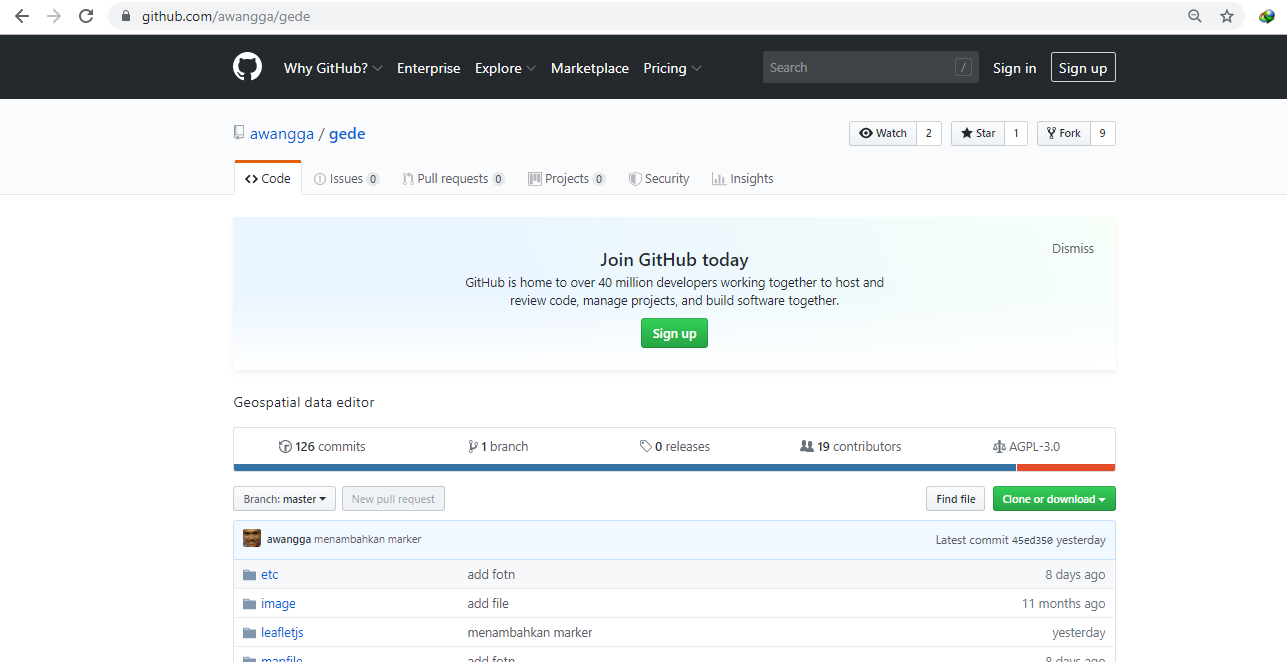
\includegraphics[width=6cm]{figures/Tugas4/1174071/5.png}
			\centering
			\caption{Download repository gede}
		\end{figure}
	\item Extrack repository gede yang telah di download
		\begin{figure}[H]
			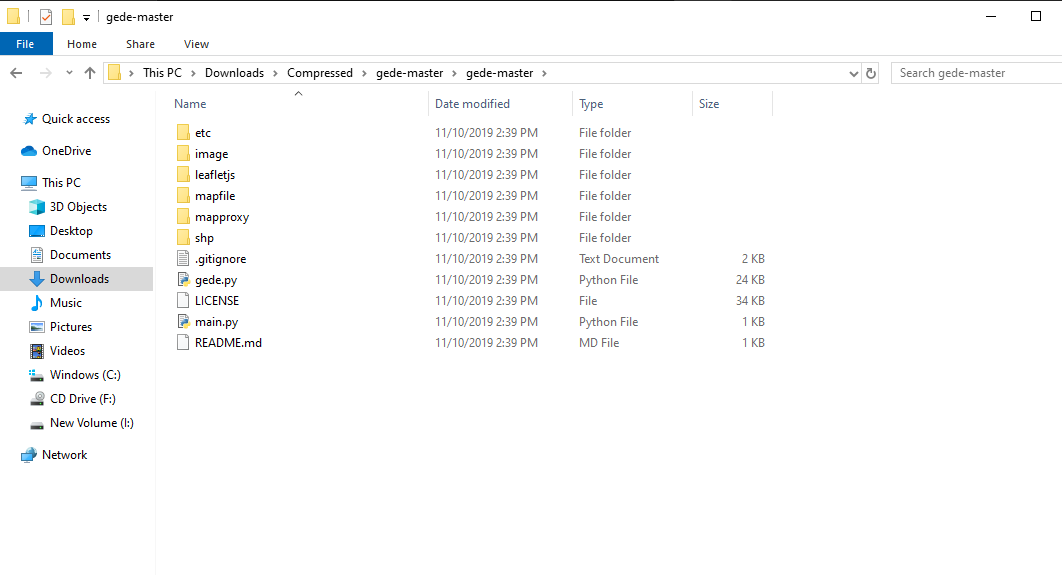
\includegraphics[width=6cm]{figures/Tugas4/1174071/6.png}
			\centering
			\caption{Extract repository}
		\end{figure}
	\item Buka folder shp pada repository gede
		\begin{figure}[H]
			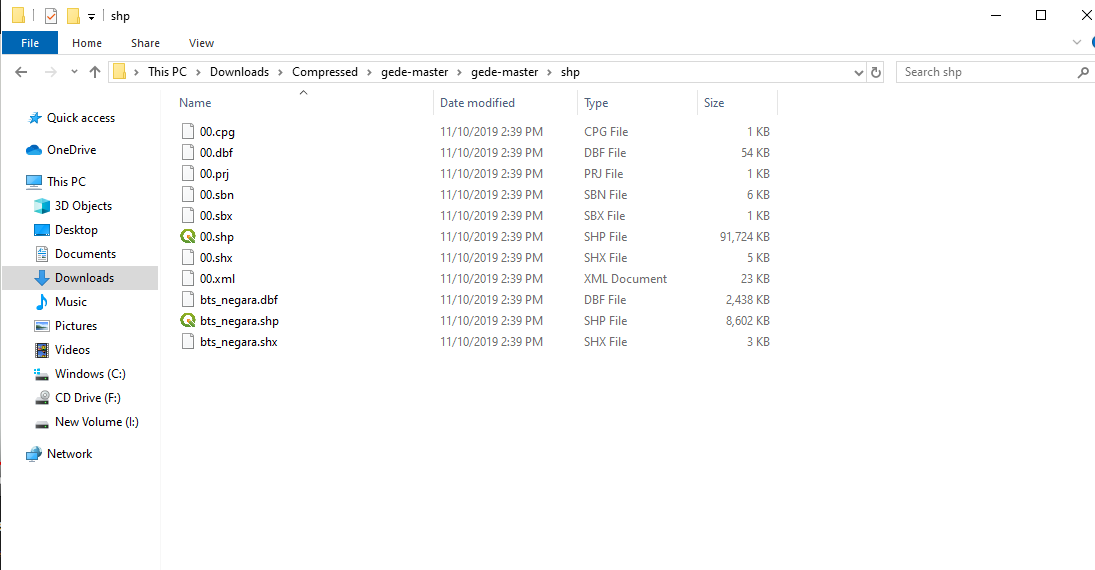
\includegraphics[width=6cm]{figures/Tugas4/1174071/7.png}
			\centering
			\caption{Buka folder shp}
			\end{figure}
	\item Buka file 00.shp menggunakan aplikasi QGIS
		\begin{figure}[H]
			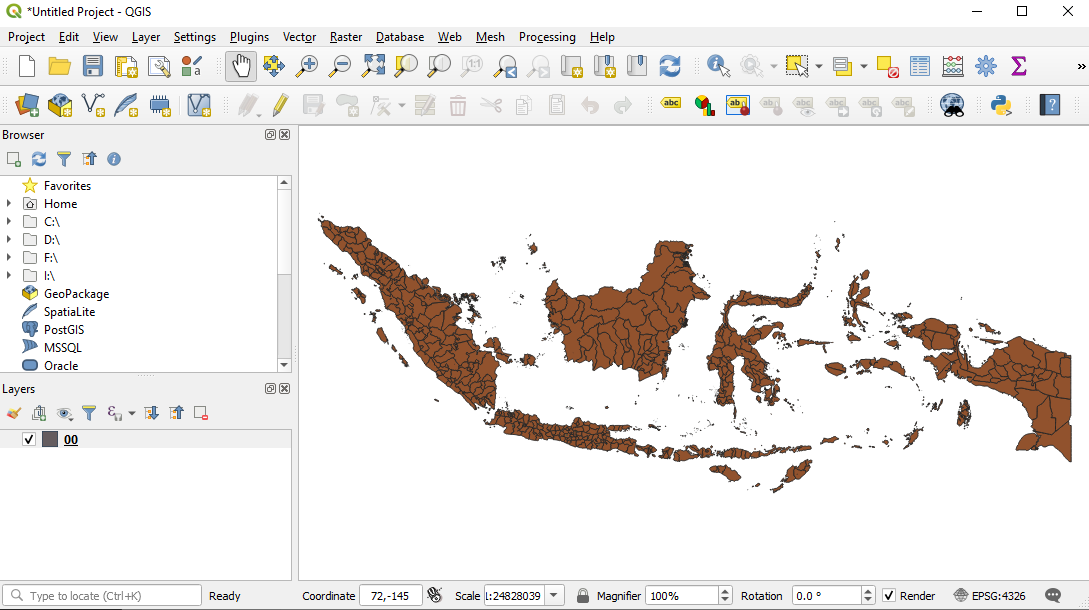
\includegraphics[width=6cm]{figures/Tugas4/1174071/8.png}
			\centering
			\caption{Hasil gambar 00.shp Negara Indonesia}
		\end{figure}
	\item Buka file btsnegara.shp menggunakan aplikasi QGIS
		\begin{figure}[H]
			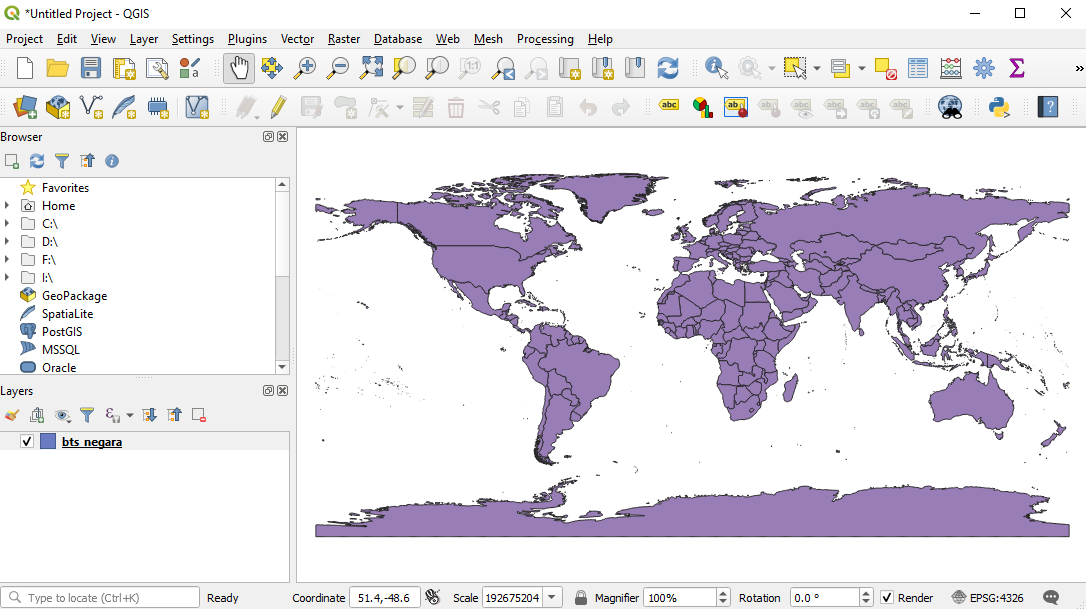
\includegraphics[width=6cm]{figures/Tugas4/1174071/9.png}
			\centering
			\caption{Hasil gambar btsnegara.shp peta dunia}
		\end{figure}
	\item Buka file 00.shp dan btsnegara.shp bersamaan menggunakan aplikasi QGIS
		\begin{figure}[H]
			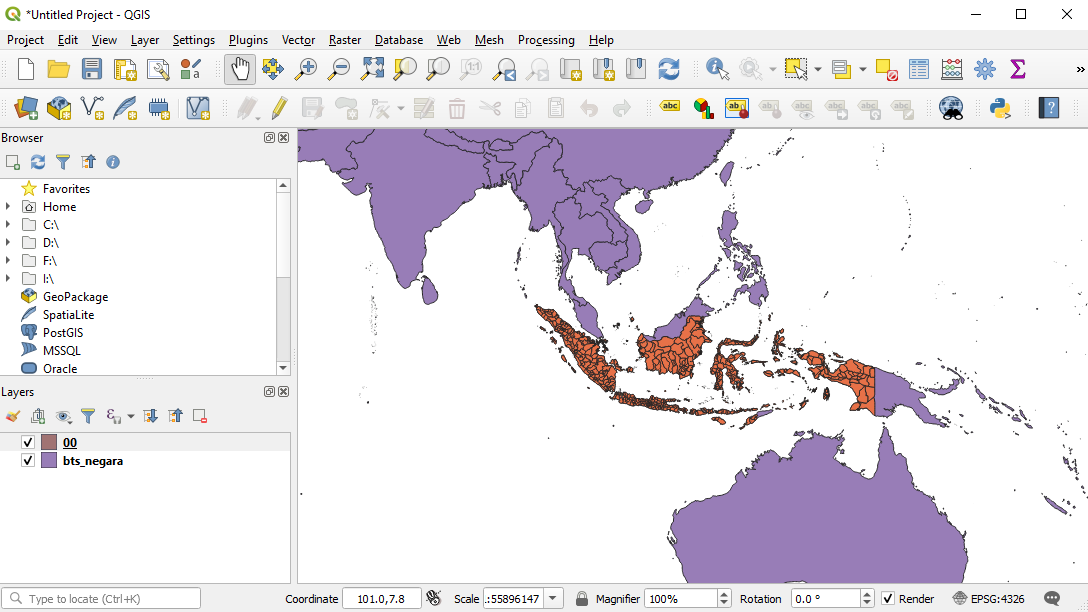
\includegraphics[width=6cm]{figures/Tugas4/1174071/10.png}
			\centering
			\caption{Hasil 00.shp dan btsnegara.shp peta dunia dengan batas negara Indonesia}
		\end{figure}
	\item Buka folder mapproxy
		\begin{figure}[H]
			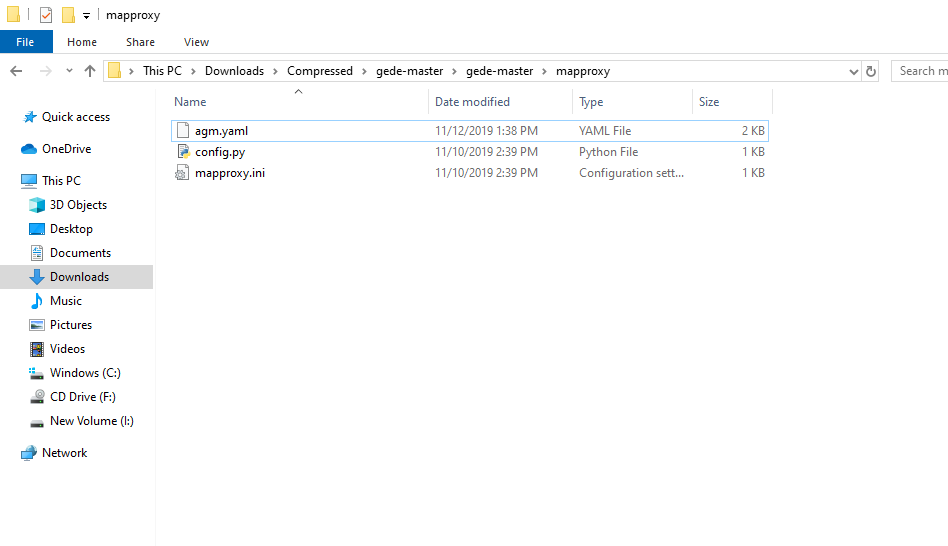
\includegraphics[width=6cm]{figures/Tugas4/1174071/11.png}
			\centering
			\caption{Isi folder mapproxy}
		\end{figure}
	\item Buka file agm.yaml menggunakan text editor lalu konfigurasikan
		\begin{figure}[H]
			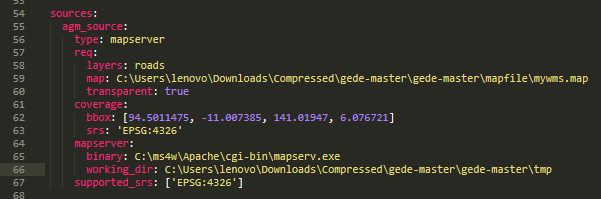
\includegraphics[width=6cm]{figures/Tugas4/1174071/12.png}
			\centering
			\caption{Konfigurasi map:lokasi file mwmys.map, binary:lokasi instal MS4C, dan workingdir:lokasi folder tmp di dalam folder gede }
		\end{figure}
	\item Jalankan map proxy dengan perintah 'mapproxy-util serve-develop agm.yaml' MS4W console shell
		\begin{figure}[H]
			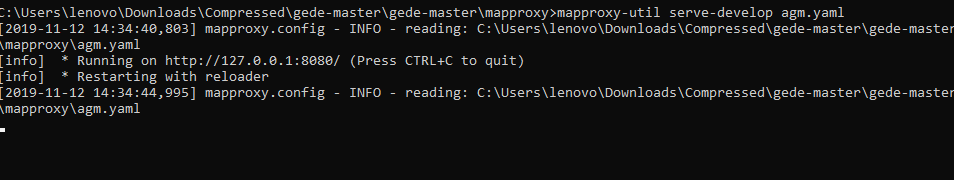
\includegraphics[width=6cm]{figures/Tugas4/1174071/13.png}
			\centering
			\caption{Jalankan map server}
		\end{figure}
	\item Buka 127.0.0.1:8080 pada browser lalu klik demo
		\begin{figure}[H]
			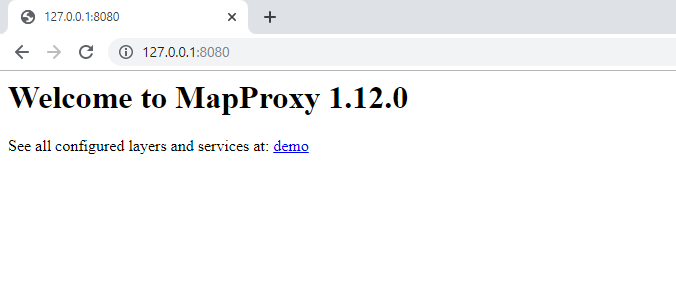
\includegraphics[width=6cm]{figures/Tugas4/1174071/14.png}
			\centering
			\caption{Buka mapproxy pada browser}
		\end{figure}
	\item Pilih salah satu png atau jpg
		\begin{figure}[H]
			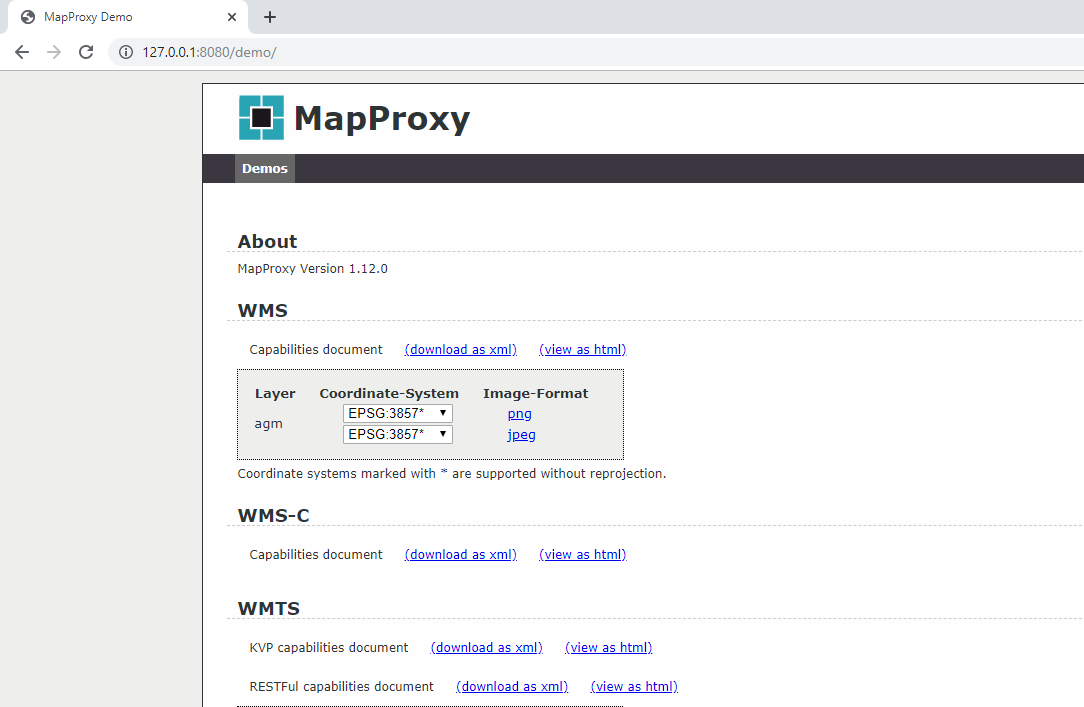
\includegraphics[width=6cm]{figures/Tugas4/1174071/15.png}
			\centering
			\caption{Pilih png atau jpg}
		\end{figure}
	\item Hasil dari mapproxy
		\begin{figure}[H]
			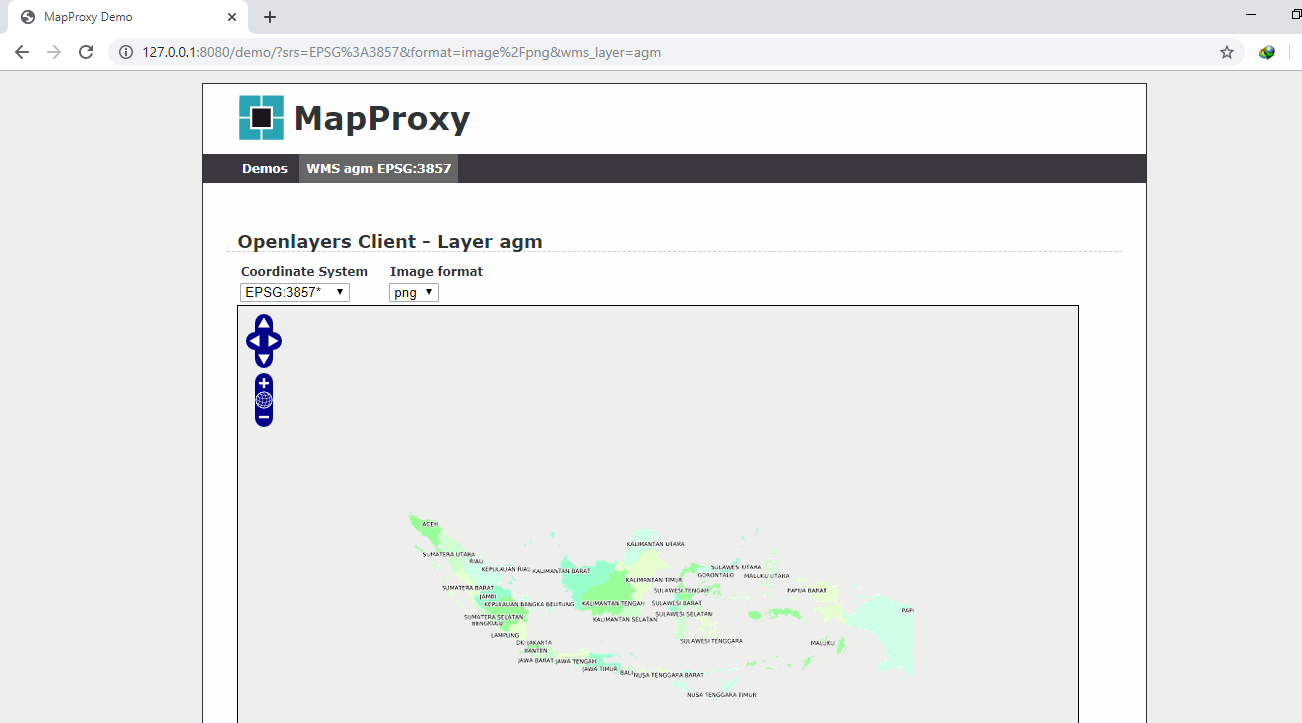
\includegraphics[width=6cm]{figures/Tugas4/1174071/16.png}
			\centering
			\caption{Hasil mapproxy}
		\end{figure}
\end{enumerate}


\subsection{Link tutorial}
https://youtu.be/sJrSy9K-7Tc
